\graphicspath{{./figures/pipeline/}}

\chapter{Data Pipeline}
We developed a pipeline (fig. \ref{fig:project_pipeline}) comprising (1) a data engineering pipeline, and (2) a data science pipeline).
We devoted significant part of our effort into following existing and developing best practices in data science development standards, so as to ensure reproducibility of results as well as reusability of methods and tools.
One of the key Python frameworks we used to attain that is the McKinsey's Kedro \cite{kedro}.

\begin{figure}[H]
	\centering
    \caption{The project pipeline.}
    \includegraphics[width=0.8\linewidth,trim={7cm 7cm 7cm 2cm},clip]{pipeline_project.pdf}
    %\includesvg{pipeline_project}
	\label{fig:project_pipeline}
\end{figure}


\section{Data Engineering Pipeline}
The data engineering pipeline (fig. \ref{fig:pipeline_de}) encompasses all the data processing steps involved between (a) measurements and sensors datasets and (b) daily capacity factors, sensors graph inputs.

\begin{figure}[H]
	\centering
    \caption{The data engineering pipeline.}
    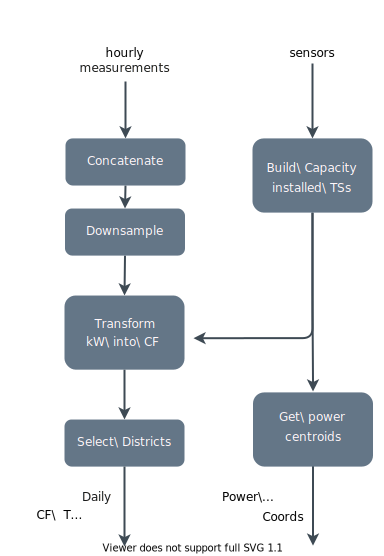
\includegraphics[width=1.0\linewidth,trim={7cm 7cm 7cm 0cm},clip]{pipeline_de.pdf}
    %\includesvg{pipeline_project}
	\label{fig:pipeline_de}
\end{figure}

\vspace{1em}
\noindent
\textbf{Get Capacity Installed Time Series.}  We load the sensors dataset and build a time series for the capacity installed in every district, essentially by grouping  turbine entries by district, and performing a cumulated sum of power ratings over the commissioning date-sorted entries.

\vspace{1em}
\noindent
\textbf{Get Power Centroids.}  A centroid position is defined for every district, not by its baricenter, but from the rated power-weighted average of all its single turbines coordinates. In practice, the power centroid changes its position every time  a new turbine is commissioned. We neglect this variation over time, and take the resulting average as sufficiently accurate for its purpose. Namely, we use the power centroids for calculating representative Euclidean distances between districts, which we used for the EDA and also when calculating the adjacency matrix initialization values for the graph-based spatio-temporal forecasting methods.

\vspace{1em}
\noindent
\textbf{Concatenate and Downsample.}  We concatenate the measurements dataset (power generated districtwise, in $kW$), which is provided for every year, into a single hourly dataframe, then downsample it into a daily measurements by summing same-day entries.

\vspace{1em}
\noindent
\textbf{Filter Districts.}   We filter out previously determined districts  which either represent outliers in spatial correlogram (3 from 303) or have zero installed capacity by 2015-01-01 (4 from 303).
Also, districts in which by 2000-01-01 a single turbine represents more than 50\% of its installed capacity (18 districts in total).
Although the latter measure might represent a deviation from the industry use case, we perform it in favor of metrics representativity, as otherwise models overall performance metrics would be biased by low predictibility of ill-conditioned time series e.g. from districts where wind harvesting are still in early phases.

\vspace{1em}
\noindent
\textbf{Transform kW to CF.}  Every entry in measurements time series dataset is normalized by the corresponding local installed capacity at the same day.
This results in daily time series for capacity factors in every district.

\pagebreak

\section{Data Science Pipeline}
The data science pipeline (fig. \ref{fig:ds-pipeline}) processes (a) user-defined parameters, (b) the capacity factors dataset resulting from the data engineering pipeline and, when required, also (c) the power centroids.

\vspace{1em}
\noindent
\textbf{Get Initial Adjacency Matrix.}  We calculate the matrix of the pairwise Euclidean distances and transform it into an adjacency matrix.
For initializing the values of the (constant) adjacency matrix in DCRNN or the self-adaptive adjacency matrix in the Graph WaveNet case, we follow the procedure in \cite{li2018dcrnn, wu2019graphwavenet} apply the Gaussian Kernel on the distances matrix, so that $A_{ij} = exp(-D_{ij}^2/2\sigma_{D}^2)$, where $\sigma_{D}$ is the standard deviation of the distances matrix.
Also as in \cite{DCRNN}, we promote sparsity in the adjacency matrix for computational efficiency by thresholding the entries in the adjacency matrix.
However, instead of defining an arbitrary threshold value for $A_{ij}$, we prune adjacency values when the distances they are calculated from surpasses the decorrelation distance of 150 km.
This node function is only processed in experiments with DCRNN and Graph WaveNet, as they are the only methods considered which rely on an adjacency matrix.

\vspace{1em}
\noindent
\textbf{Split Inference-Test Data.}  We split the capacity factors measurements dataset into a model inference dataset, used for training and model selection, and a test dataset, reserved for the model performance evaluation.
The split is done according to the user-defined date ranges defined for each partition.

\vspace{1em}
\noindent
\textbf{Scale.}  We apply the user-defined sequence of scaling and offsetting methods on the inference data.

\vspace{1em}
\noindent
\textbf{Define CV Splits Positions.}  Date ranges for defining respectively the training and the validation datasets are determined, the validation window always positioned on dates later than training window last entry.
User-defined entries for this function include the cross-validation scheme and the pertaining parameters.
For expanding window CV, the parameters are the relative size of the shortest train window (0.0 - 1.0 proportion of model inference dataset size), the number of total CV passes, the number of steps ahead, and the forecast window size.

\vspace{1em}
\noindent
\textbf{CV Train.}  Trains a model for every CV split as well as one for the entire scaled model inference dataset.
In the case of single time series-modeling methods such as Holt-Winters Exponential Smoothing, the resulting model is actually a simple collection of single time series submodels.

\vspace{1em}
\noindent
\textbf{Evaluate.}  Makes predictions using every trained model in the experiment and calculate overall model performance metrics.